\documentclass[11pt,letterpaper]{article}
\PassOptionsToPackage{hyphens}{url}
\usepackage[margin=.83in,top=.8in,bottom=.8in,headheight=15pt]{geometry}
\usepackage[T1]{fontenc}
\usepackage{lmodern,amsmath,amssymb,mathtools,bm,booktabs,array,graphicx,tikz}
\usetikzlibrary{arrows.meta,positioning,calc,decorations.pathreplacing,patterns}
\definecolor{ink}{HTML}{17344D}\definecolor{accent}{HTML}{087E8B}\definecolor{pale}{HTML}{EDF5F5}\definecolor{gold}{HTML}{AD6B19}
\providecommand{\dd}{\,\mathrm{d}}\providecommand{\R}{\mathbb{R}}
\providecommand{\E}{\mathbb{E}}\providecommand{\Var}{\operatorname{Var}}
\providecommand{\Cov}{\operatorname{Cov}}\providecommand{\diag}{\operatorname{diag}}
\providecommand{\norm}[1]{\left\lVert#1\right\rVert}
\providecommand{\abs}[1]{\left|#1\right|}
\usepackage{microtype,hyperref,fancyhdr,enumitem,amsthm,sectsty,needspace}
\allsectionsfont{\raggedright}
\hypersetup{colorlinks=true,linkcolor=ink,urlcolor=accent,pdfauthor={Zan Ahmad},pdftitle={Circulatory models and parameter identifiability / Lecture notes}}
\setlength{\parindent}{0pt}\setlength{\parskip}{6pt}\linespread{1.07}
\setlist{itemsep=3pt,topsep=4pt,leftmargin=*}
\emergencystretch=2em\clubpenalty=10000\widowpenalty=10000
\pagestyle{fancy}\fancyhf{}\fancyhead[L]{\small Computational Cardiology}\fancyhead[R]{\small Lecture 1}
\fancyfoot[L]{\footnotesize Zan Ahmad}\fancyfoot[R]{\footnotesize\thepage}\renewcommand{\headrulewidth}{.3pt}
\newtheorem{proposition}{Proposition}\newtheorem{theorem}{Theorem}\newtheorem{lemma}{Lemma}
\theoremstyle{definition}\newtheorem{definition}{Definition}\newtheorem{example}{Example}
\numberwithin{equation}{section}
\begin{document}
{\small\scshape Computational Cardiology\hfill Lecture 1}\par\medskip
{\raggedright\hyphenpenalty=10000\exhyphenpenalty=10000\LARGE\bfseries\color{ink} Circulatory models and parameter identifiability\par}\medskip
{\small Lecture notes}\par\bigskip
A circulation model relates quantities that can be prescribed or measured to quantities that must be inferred. We begin with conservation of blood volume, distinguish the two pressure differences that enter a lumped model, and derive the information contained in a mean-flow observation. Even this small example has a nontrivial inverse problem: an exactly fitted output can correspond to an entire family of physiological parameters.

\section{Model resolution and measurable quantities}
\hypertarget{note-model-resolution-and-measurable-quantities}{}\label{note:model-resolution-and-measurable-quantities}
{\small \href{slides.html\#frame=states-and-observations\&step=1}{Slides for this section}}\par
A resistance network resolves mean transport. A pulsatile compartment model additionally resolves storage, pressure waveforms and valve events. A spatial mechanics model resolves deformation and stress. These descriptions retain different information; their predictions cannot be compared with an observation that the chosen state space does not represent.

For mean perfusion, averaging over beats may be appropriate. For valve timing, the averaging would remove the event of interest. For local wall stress, spatial geometry, material response and loading must enter the model. Geometry alone does not identify uncertain material parameters. The observable therefore determines which distinctions the model must retain.

A useful notation separates dynamics from observation:
\[
 \dot x=F(x,\vartheta,u),\qquad y=H(x,\vartheta,u).
\]
Here $x$ is the state, $\vartheta$ the parameter vector, $u$ a prescribed input and $y$ the predicted observation. Specifying $H$ is part of specifying the model. A pressure waveform, a beat-averaged flow and a spatial wall-stress field are different observations, even when they arise from the same experiment. A state space containing only compartment volumes cannot produce a resolved wall-stress field without an additional spatial model.
\section{A closed circulation as a directed network}
\hypertarget{note-a-closed-circulation-as-a-directed-network}{}\label{note:a-closed-circulation-as-a-directed-network}
{\small \href{slides.html\#frame=the-two-pump-circuit\&step=1}{Slides for this section}}\par
Blood leaving the left ventricle enters systemic arteries, passes through systemic tissues, returns through systemic veins to the right heart, traverses the lungs, and returns through pulmonary veins to the left heart. The circulation diagram groups that path into six storage regions: two ventricles and four vascular regions. It omits atrial storage as a separate state, spatial gradients inside each region, regional organ branches, and detailed vessel geometry. A model box is therefore not an additional anatomical heart chamber. The pressures refer to these functional storage regions.

The four ideal valve links identify mitral, aortic, tricuspid and pulmonic pathways. The two vascular beds supply systemic and pulmonary resistance. The topology distinguishes the two pumps and two circulations, while the closed outer boundary declares that this model has no transfusion, bleeding or external blood reservoir. Each internal transfer leaves one region and enters another. Summing the volume balances must cancel every such transfer; if it does not, either the boundary or the implementation is inconsistent.

The actual heart is active. A passive closed resistor network without an energy source cannot sustain circulation. The later compartment model represents pumping by changing ventricular compliance during a shared cardiac cycle. That is a constitutive assumption, not an explanation of muscle activation. The present meeting establishes which quantities that representation can expose; it does not yet derive the valve-switching pressure solver.

Orient every internal edge from its upstream region to its downstream region. Let $B_{ie}=+1$ at the receiving compartment, $B_{ie}=-1$ at the donating compartment, and zero elsewhere. The volume balances are
\[
 \dot{\boldsymbol V}=B\boldsymbol q,
 \qquad \boldsymbol 1^{\mathsf T}B=0,
 \qquad \frac{\mathrm d}{\mathrm dt}\sum_i V_i=0.
\]
The last identity follows from topology, independently of the constitutive laws used to compute the edge flows. An external source would instead add a vector $s$ and produce $\mathrm d\sum_iV_i/\mathrm dt=\sum_i s_i$.
\begin{center}\begin{minipage}{.98\linewidth}\centering
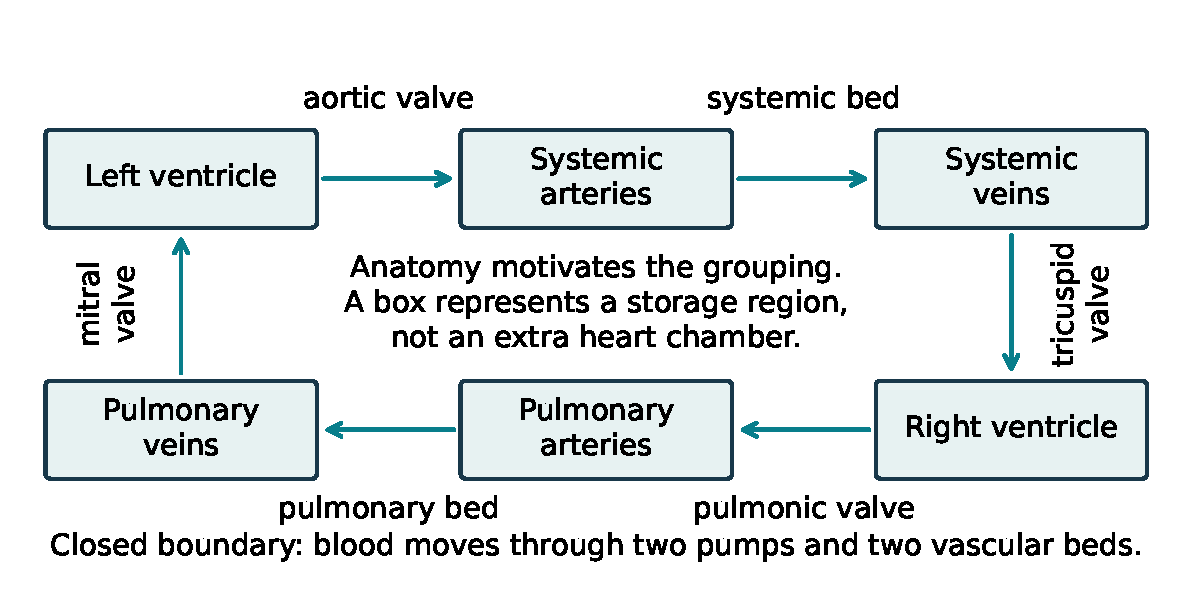
\includegraphics[width=.96\linewidth,height=.57\textheight,keepaspectratio]{circulation-map.pdf}\par\smallskip
{\small Original functional grouping for a closed two-pump circuit. Four ideal valve links and two vascular beds connect the regions.}
\end{minipage}\end{center}
\section{Pressure, storage and physical units}
\hypertarget{note-pressure-storage-and-physical-units}{}\label{note:pressure-storage-and-physical-units}
{\small \href{slides.html\#frame=flow-and-compliant-storage\&step=1}{Slides for this section}}\par
A state is information needed to continue the model: stored volumes, or pressures when a specified compliance relates pressure and volume. Parameters specify relationships, such as resistance or an unstressed volume. Inputs are prescribed conditions or interventions. Observations are measurements compared with predictions. The same named physical quantity can play different roles in different experiments: an endpoint pressure may be prescribed in a bench experiment or predicted in a closed circulation. State the role explicitly instead of relying on variable names.

Pressure has two distinct uses. The difference between two fluid pressures drives an open-resistor flow. Pressure relative to surrounding tissue is the transmural pressure used in a compliance law. If both interior and exterior gauges shift consistently, the physical transmural pressure is unchanged. If the exterior stays fixed while the interior rises, stored volume may change. A gauge argument that preserves flow does not justify leaving vessel volume unchanged under that second intervention.

Units prevent a model boundary from disappearing inside a formula. Use liters for volume, minutes for hydraulic time and mmHg for pressure. Resistance then has units mmHg min/L; compliance has L/mmHg. Heart rate in beats/min multiplied by stroke volume in mL/beat gives mL/min, requiring division by 1000 for L/min. The word beat cancels as an event count, while the distinction between minutes and seconds remains essential.

For an open resistive connection and a linear compliant compartment, respectively,
\[
 q_{ij}=\frac{P_i-P_j}{R_{ij}},\qquad
 V_i=V_{0i}+C_i(P_i-P_{{\rm ext},i}).
\]
Adding the same constant to both fluid pressures leaves $q_{ij}$ unchanged. The storage relation is unchanged only if the exterior pressure is shifted as well. The dimensions are
\[
 [R]=\frac{\mathrm{mmHg}\,\mathrm{min}}{\mathrm L},\qquad
 [C]=\frac{\mathrm L}{\mathrm{mmHg}},\qquad [RC]=\mathrm{min}.
\]
Thus the product $RC$ already has the dimensions of a relaxation time.
\section{Mean flow as an observation map}
\hypertarget{note-mean-flow-as-an-observation-map}{}\label{note:mean-flow-as-an-observation-map}
{\small \href{slides.html\#frame=transport-over-repeated-beats\&step=1}{Slides for this section}}\par
For repeated beats at a fixed rate, define stroke volume as the net forward volume delivered per beat over the chosen averaging window. Mean cardiac output is heart rate times stroke volume. This identity requires a compatible window and convention; during changing rate or unequal successive beats, average the actual transported volume over elapsed time. Multiplying two separately averaged quantities need not reproduce that transport. We use a constant-rate example so that the simple product is exact within its stated bookkeeping model.

Take a synthetic mean output of 6 L/min and a systemic pressure drop of 90 mmHg. A mean open-resistance description gives an effective resistance of 15 mmHg min/L. Three candidate pairs produce the same output: 60 beats/min with 100 mL/beat, 80 with 75, and 120 with 50. All three also produce the same inferred resistance from these observations. The agreement is a consequence of the observation map, not evidence that the underlying pulsatile states are equivalent.

The plotted curve contains every positive pair whose product is 6000 mL/min. Moving along it changes rate and stroke volume without changing the measured mean output. A single scalar observation therefore cannot determine two freely varying factors. Knowing rate independently would permit stroke volume to be inferred under the product assumption; it would still not reveal ventricular pressure shape, valve leakage or spatial flow structure.

\[
\overline Q=F\,SV/1000
\]
This product is used for a repeated constant-rate cycle.

\[
R_{\rm eff}=\Delta\overline P/\overline Q
\]
Resistance has units mmHg min/L.

For $n$ identical beats in an elapsed time $T$, the transported volume is $n\,SV$ and $F=n/T$. Dividing volume by elapsed time gives the mean-flow formula. For unequal beat volumes $SV_k$, the more general expression is
\[
 \overline Q=\frac{1}{1000T}\sum_{k=1}^{n}SV_k,
\]
with $T$ in minutes and each $SV_k$ in mL. The product of separately chosen time averages is not a replacement for this transport balance.

\paragraph{Calculation.} Two candidates have rates 60 and 120 beats/min and stroke volumes 100 and 50 mL/beat. The measured pressure drop is 90 mmHg.

Both products are 6000 mL/min, or 6 L/min.

Both imply effective resistance 90/6 = 15 mmHg min/L.

The two observations do not distinguish the candidates; measuring rate supplies different information.

An exact fit need not identify the hidden factors.
\begin{center}\begin{minipage}{.98\linewidth}\centering
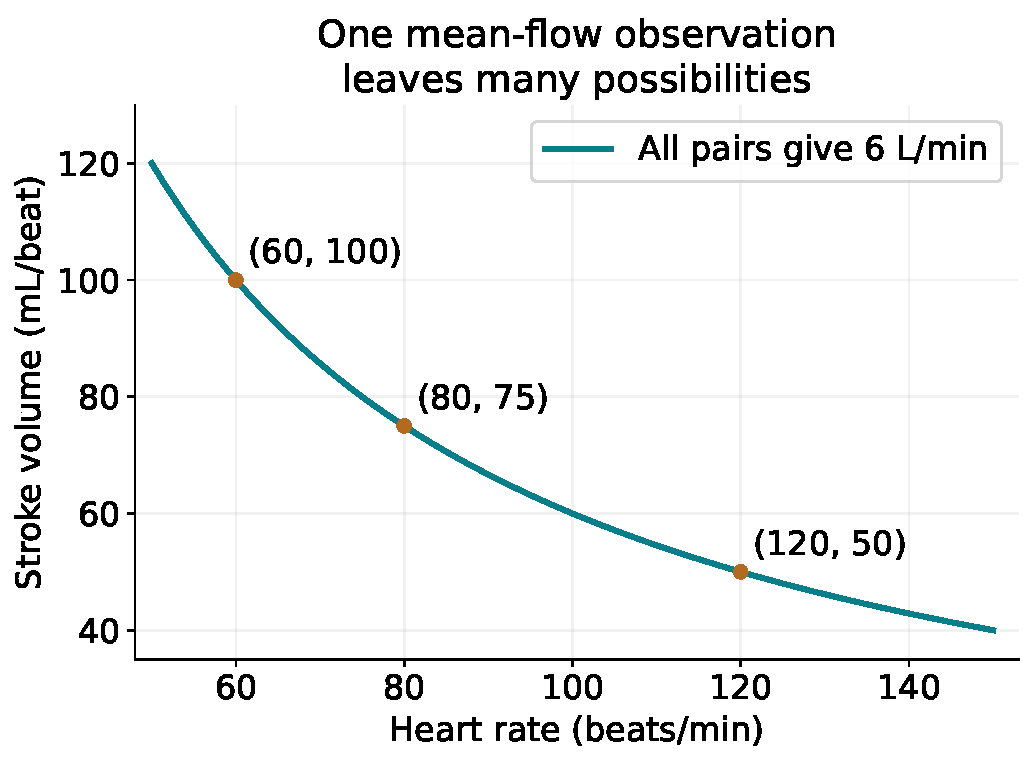
\includegraphics[width=.96\linewidth,height=.57\textheight,keepaspectratio]{flow-identifiability.pdf}\par\smallskip
{\small Synthetic constant-rate pairs all produce 6 L/min. The curve demonstrates a missing independent constraint, not a clinical relationship between rate and stroke volume.}
\end{minipage}\end{center}
\section{Parameter symmetries and local identifiability}
\hypertarget{note-parameter-symmetries-and-local-identifiability}{}\label{note:parameter-symmetries-and-local-identifiability}
{\small \href{slides.html\#frame=an-exact-parameter-symmetry\&step=1}{Slides for this section}}\par
The small-change calculation makes the ambiguity explicit. Differentiate the product: a flow change equals stroke volume times the rate change plus rate times the stroke-volume change, divided by 1000. At one operating point this is one equation for two changes. Opposite relative changes cancel to first order. A finite product-preserving change multiplies rate by a positive factor and divides stroke volume by the same factor. The companion tests this exact symmetry rather than relying only on a plotted coincidence.

An optimization routine can still return one parameter pair if you ask it to fit mean flow alone. Its numerical success does not remove the ambiguity; bounds, initialization or regularization may select the reported point. State which additional information makes the selection meaningful. A rate measurement, an independently measured stroke volume, or a richer waveform can constrain different aspects. Measurement uncertainty then affects how precisely those quantities can be distinguished. More samples of the identical uninformative observable do not automatically add a missing independent constraint.

\[
\delta\overline Q=(SV\,\delta F+F\,\delta SV)/1000
\]
This is a local first-order relation; exact finite invariance uses F multiplied and SV divided by the same factor.

Write $H(F,SV)=F\,SV/1000$. For every $a>0$,
\[
 H(aF,SV/a)=H(F,SV).
\]
Consequently, the inverse image of a positive observation $Q_0$ is the curve $SV=1000Q_0/F$, rather than a single point. The differential has rank one:
\[
 DH=\frac1{1000}\begin{pmatrix}SV&F\end{pmatrix},
 \qquad DH\begin{pmatrix}F\\-SV\end{pmatrix}=0.
\]
The null vector is tangent to the family of indistinguishable parameters. In relative variables, $\delta Q/Q=\delta F/F+\delta SV/SV$, so opposite relative perturbations cancel to first order.
\section{Independent observations and model error}
\hypertarget{note-independent-observations-and-model-error}{}\label{note:independent-observations-and-model-error}
{\small \href{slides.html\#frame=adding-an-independent-measurement\&step=1}{Slides for this section}}\par
Verification asks whether code implements the chosen equations. Here dimensional conversion, product-preserving changes and limiting input rejection are direct checks. In the later closed circulation, total-volume balance and valve consistency add independent constraints. A computed answer can pass those checks while an important physical mechanism is absent. Validation asks whether predictions agree with observations appropriate to the intended use, with uncertainty and measurement definitions stated.

If heart rate is measured independently, use the augmented map
\[
 \widetilde H(F,SV)=\begin{pmatrix}F\,SV/1000\\F\end{pmatrix},
 \qquad
 D\widetilde H=\begin{pmatrix}SV/1000&F/1000\\1&0\end{pmatrix}.
\]
Its determinant is $-F/1000$, which is nonzero for $F>0$. The inverse is then explicit: $SV=1000Q/F$. For small measurement errors,
\[
 \frac{\delta SV}{SV}\simeq\frac{\delta Q}{Q}-\frac{\delta F}{F}.
\]
This calculation removes the two-parameter ambiguity, but it does not recover an unobserved pressure waveform. A richer state model would require observations sensitive to the additional state variables. Numerical conservation, identifiable parameters and agreement with independent physical observations address distinct parts of that inference.
\bigskip
\section*{Exercises}
\par\noindent\begin{minipage}{\linewidth}
\subsection*{A1-1. Audit a mean-flow inference}
A synthetic repeated cycle has F=\allowbreak{}75 beats/min, SV=\allowbreak{}64 mL/beat and mean systemic pressure drop 84 mmHg.

\textbf{a} Calculate mean flow with units.

\end{minipage}\par\medskip
\textbf{b} Calculate effective resistance and state one omitted mechanism.

\textbf{c} Would matching this resistance establish the correct ventricular waveform?

\par\noindent\begin{minipage}{\linewidth}
\subsection*{A1-2. Choose a boundary and observable}
Compare a question about mean systemic perfusion with one about the location of peak ventricular wall stress.

\textbf{a} Propose the minimum useful model level and an observable for each.

\end{minipage}\par\medskip
\textbf{b} Name a mechanism omitted by the first model that matters to the second.

\textbf{c} Give one numerical check and one additional observation for the first model.

\par\noindent\begin{minipage}{\linewidth}
\subsection*{A1-3. Expose a hidden ambiguity}
Candidates A and B have (F,SV)=\allowbreak{}(60,80) and (80,60), with rate in beats/min and stroke volume in mL/beat.

\textbf{a} Show whether mean flow distinguishes the candidates.

\end{minipage}\par\medskip
\textbf{b} Apply the finite transformation F$\to$1.25F and SV$\to$SV/1.25 to candidate A.

\textbf{c} Select a new measurement and explain what remains unresolved.

\section*{References}
\noindent\begin{minipage}{\linewidth}
Zan Ahmad, Advanced Topics in Computational Cardiology syllabus, Fall 2024. PDF pages 1--2.

\end{minipage}\par\medskip
\noindent\begin{minipage}{\linewidth}
Hoppensteadt and Peskin, Modeling and Simulation in Medicine and the Life Sciences, second edition. Printed pages 5--10; supplied PDF pages 18--23.

\end{minipage}\par\medskip
\end{document}
